\documentclass[review]{elsarticle}

\usepackage{natbib}
\usepackage{graphicx, subfigure}
\usepackage{dcolumn}% Align table columns on decimal point
\usepackage{bm}% bold math

%\usepackage{lineno,hyperref, url}
\usepackage{indentfirst}
\usepackage{array, threeparttable}
\usepackage{multirow}
\usepackage{mathrsfs}
\usepackage{color}
\usepackage{amsmath, amssymb}

%\modulolinenumbers[5]

\journal{Journal of \LaTeX\ Templates}

%%%%%%%%%%%%%%%%%%%%%%%
%% Elsevier bibliography styles
%%%%%%%%%%%%%%%%%%%%%%%
%% To change the style, put a % in front of the second line of the current style and
%% remove the % from the second line of the style you would like to use.
%%%%%%%%%%%%%%%%%%%%%%%

%% Numbered
%\bibliographystyle{model1-num-names}

%% Numbered without titles
%\bibliographystyle{model1a-num-names}

%% Harvard
%\bibliographystyle{model2-names.bst}\biboptions{authoryear}

%% Vancouver numbered
%\usepackage{numcompress}\bibliographystyle{model3-num-names}

%% Vancouver name/year
%\usepackage{numcompress}\bibliographystyle{model4-names}\biboptions{authoryear}

%% APA style
%\bibliographystyle{model5-names}\biboptions{authoryear}

%% AMA style
%\usepackage{numcompress}\bibliographystyle{model6-num-names}

%% `Elsevier LaTeX' style
\bibliographystyle{elsarticle-num}
%%%%%%%%%%%%%%%%%%%%%%%

\begin{document}

\begin{frontmatter}

\title{The transformation of coordinate system}
\tnotetext[mytitlenote]{The Notes of coordinate system transform.}

\author[mysecondaryaddress]{Ji Li\corref{mycorrespondingauthor}}
\fntext[myfoootnote]{A study notes.}
\cortext[mycorrespondingauthor]{Corresponding author}
\ead{leejearl@126.com}
\address{National Key Laboratory of Science and Technology on Aerodynamic Design and Research, Northwestern Polytechnical University, Xi'an, Shaanxi 710072, China}
\begin{abstract}
	Some important notes for the transformation of coordinate system.
\end{abstract}

\begin{keyword}
	Transformation of coordinate system, Scalar, Vector, Partial derivatives.
\end{keyword}

\end{frontmatter}

%\linenumbers

\section{Definition of coordinate system}
The original coordinate system is defined as $x\sim y$. The new coordinate system is $x' \sim y'$, which 
is obtained by rotating $x \sim y$ for $\theta$ degree. Fig.~\ref{fig:CoordinateSystemRotation} shows the relations of two coordinate systems. 

\begin{figure}[!htp]
	\centering
	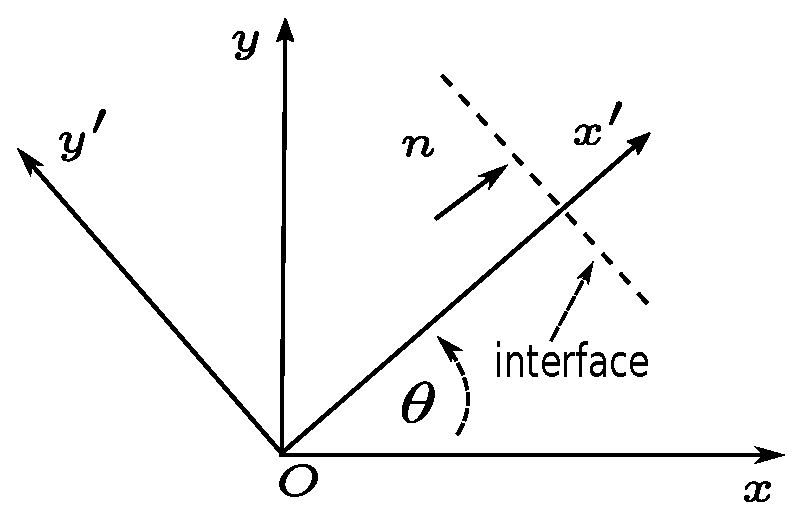
\includegraphics[width=0.5\textwidth]{CoordinateSystemRotation.eps}
	\caption{The relations of $x \sim y$ and $x' \sim y'$}.
	\label{fig:CoordinateSystemRotation}
\end{figure}

The scalar variables in $x \sim y$ and $x' \sim y'$ are expressed as $p$ and $p'$ respectively. The vector variables in $x \sim y$ and $x' \sim y'$ are read as $\bm{u}$ and $\bm{u}'$ respectively.
The unit normal vector of $x'-\text{axis}$ under $x \sim y$ can be expressed as
\begin{equation}\label{normal}
	\bm{n}=(n_x, n_y) = (cos\theta, sin\theta).\\
\end{equation}
The unit normal vector of $y'-\text{axis}$ under $x \sim y$ is
\begin{equation}\label{tangent}
	\bm{t} = (t_x, t_y) = (-n_y, n_x)=(-sin\theta, cos\theta).
\end{equation}

\section{Transformation of variables}
\begin{itemize}
	\item Scalar variables\\
		\begin{equation}\label{scalarTransformation}
			p'=p.
		\end{equation}
	\item Vector variables\\
		Let 
		\begin{equation}\label{vector_u}
			\bm{u}=(u, v)^T,\quad \bm{u}'=(u', v')^T,
		\end{equation}
		thus,
		\begin{equation}\label{vectorTransformation}
			\bm{u}'=\left(
				\begin{array}{c}
					\bm{n} \\
					\bm{t}
				\end{array}
			\right)\bm{u}.
		\end{equation}
\end{itemize}

\section{Directional derivative}
We assume that the unit directional derivative $\bm{l}$ has the following form
\begin{equation}\label{vector_l}
	\bm{l}=(l_x, l_y)^T,
\end{equation}
thus, the directional derivative of scalar and vector variables under $x \sim y$ can be expressed as
\begin{equation}\label{directionalDerivatives:scalar:origin}
	\frac{\partial p}{\partial \bm{l}} = \nabla p \cdot \bm{l}, 
\end{equation}
and 
\begin{equation}\label{directionalDerivatives:vector:origin}
	\frac{\partial \bm{u}}{\partial \bm{l}} = \frac{\partial}{\partial \bm{l}}\left(\bm{u}\right)
	=\frac{\partial}{\partial \bm{l}}\left(
		\begin{array}{c}
			u\\
			v
		\end{array}
		\right).
\end{equation}\label{directionalDerivatives:scalar:new}
The scalar variables $p'$ under $x' \sim y'$ can be written as
\begin{equation}
	\frac{\partial p'}{\partial \bm{l}}=\frac{\partial p}{\partial \bm{l}} = \nabla p \cdot \bm{l}. 
\end{equation}
The vector variables $\bm{u}'$ under $x' \sim y'$ is
\begin{equation}\label{directionalDerivatives:vector:new}
	\frac{\partial \bm{u}'}{\partial \bm{l}} = \frac{\partial}{\partial \bm{l}}\left(\bm{u}'\right)
	=\frac{\partial}{\partial \bm{l}}\left(\left(
		\begin{array}{c}
			\bm{n} \\
			\bm{t}
		\end{array}
	\right)\bm{u}\right)
	=\left(
		\begin{array}{c}
			\bm{n} \\
			\bm{t}
		\end{array}
	\right)\frac{\partial}{\partial \bm{l}}\left(\bm{u}\right).
\end{equation}


\section{The partial derivative operators of unit vector}
The different order of partial derivative operators of unit vector are read as
\begin{equation}\label{partlO1}
	\begin{gathered}
		\frac{\partial}{\partial \bm{l}} = \bm{l}\cdot \nabla,\quad 
		\frac{\partial^2}{\partial \bm{l}^2} = \left(\bm{l}\cdot \nabla\right)\left(\bm{l}\cdot \nabla\right),\\
		\frac{\partial^2}{\partial \bm{l}_1\partial \bm{l}_2} = \left(\bm{l}_1\cdot \nabla\right)\left(\bm{l}_2\cdot \nabla\right),\quad 
		\frac{\partial^{m+n}}{\partial^m \bm{l}_1\partial^n \bm{l}_2} = \left(\bm{l}_1\cdot \nabla\right)^m\left(\bm{l}_2\cdot \nabla\right)^n.
	\end{gathered}
\end{equation}

\textit{\textbf{Examples:}}\\
\begin{equation}\label{partialxmyn}
	\begin{gathered}
		\frac{\partial}{\partial x'} = \frac{\partial}{\partial \bm{n}}
			=\bm{n} \cdot \nabla = n_x\frac{\partial}{\partial x}+n_y\frac{\partial}{\partial y},\\
		\frac{\partial}{\partial y'} = \frac{\partial}{\partial \bm{t}}
			=\bm{t} \cdot \nabla = -n_y\frac{\partial}{\partial x}+n_x\frac{\partial}{\partial y},\\
		\frac{\partial^2}{\partial x'^2} = \frac{\partial^2}{\partial\bm{n}^2} 
			=\left(\bm{n} \cdot \nabla\right)\left(\bm{n} \cdot \nabla\right)
			=\left(n_x\frac{\partial}{\partial x}+n_y\frac{\partial}{\partial y}\right)\left(n_x\frac{\partial}{\partial x}+n_y\frac{\partial}{\partial y}\right)\\
			=n_x^2\frac{\partial^2}{\partial x^2}+2n_xn_y\frac{\partial^2}{\partial x\partial y}+n_y^2\frac{\partial^2}{\partial y^2},\\
		\frac{\partial^2}{\partial x'\partial y'} = \frac{\partial^2}{\partial\bm{n}\partial \bm{t}} 
			=\left(\bm{n} \cdot \nabla\right)\left(\bm{t} \cdot \nabla\right)
			=\left(n_x\frac{\partial}{\partial x}+n_y\frac{\partial}{\partial y}\right)\left(-n_y\frac{\partial}{\partial x}+n_x\frac{\partial}{\partial y}\right)\\
			=n_xn_y\left(\frac{\partial^2}{\partial y^2}-\frac{\partial^2}{\partial x^2}\right)+\left(n_x^2-n_y^2\right)\frac{\partial^2}{\partial x\partial y},\\
		\frac{\partial^2}{\partial y'^2} = \frac{\partial^2}{\partial\bm{t}^2} 
			=\left(\bm{t} \cdot \nabla\right)\left(\bm{t} \cdot \nabla\right)
			=\left(-n_y\frac{\partial}{\partial x}+n_x\frac{\partial}{\partial y}\right)\left(-n_y\frac{\partial}{\partial x}+n_x\frac{\partial}{\partial y}\right)\\
			=n_y^2\frac{\partial^2}{\partial x^2}-2n_xn_y\frac{\partial^2}{\partial x\partial y}+n_x^2\frac{\partial^2}{\partial y^2}.
	\end{gathered}
\end{equation}

\section{The partial derivatives of scalar}
The procedure of transforming the partial derivatives of scalar can be considered as two stages. The first is to transform the scalar, and the second is to transform the partial derivative operator. Since the scalar is uniform under origin and transformed coordinate system, there is no need extra efforts to transform the scalar. Thus
\begin{equation}\label{dmndx'mdy'n:scalar}
	\begin{gathered}
		\frac{\partial^{m+n}p'}{\partial x'^my'^n} = \frac{\partial^{m+n}}{\partial x'^my'^n}p'
		=\frac{\partial^{m+n}}{\partial x'^my'^n}p.
	\end{gathered}
\end{equation}
\textit{\textbf{Examples:}}\\
\begin{equation}\label{dp'dx'}
	\begin{gathered}
		\frac{\partial{p'}}{\partial{x'}}
		=\left(n_x\frac{\partial}{\partial{x}} + n_y\frac{\partial}{\partial{y}}	\right)p,
	\end{gathered}
\end{equation}
\begin{equation}\label{dp'dy'}
	\begin{gathered}
		\frac{\partial{p'}}{\partial{y'}} 
		= \left(-n_y\frac{\partial}{\partial{x}} + n_x\frac{\partial}{\partial{y}} \right)p,
	\end{gathered}
\end{equation}
\begin{equation}\label{dp'2dx'2}
	\begin{gathered}
		\frac{\partial^2{p'}}{\partial{x'^2}} 
		= \left(n_x^2\frac{\partial^2}{\partial x^2}+2n_xn_y\frac{\partial^2}{\partial x\partial y}
		+n_y^2\frac{\partial^2}{\partial y^2} \right)p,
	\end{gathered}
\end{equation}
\begin{equation}\label{dp'2dx'dy'}
	\begin{gathered}
		\frac{\partial^2{p'}}{\partial{x'y'}} 
		= \left(n_xn_y\left(\frac{\partial^2}{\partial y^2}-\frac{\partial^2}{\partial x^2}\right)
		+\left(n_x^2-n_y^2\right)\frac{\partial^2}{\partial x\partial y} \right)p,
	\end{gathered}
\end{equation}
\begin{equation}\label{dp'2dy'2}
	\begin{gathered}
		\frac{\partial^2{p'}}{\partial{y'^2}} 
		= \left( n_y^2\frac{\partial^2}{\partial x^2}-2n_xn_y\frac{\partial^2}{\partial x\partial y}
		+n_x^2\frac{\partial^2}{\partial y^2}\right)p.
	\end{gathered}
\end{equation}

\section{The partial derivatives of vector}
The procedure of transforming the partial derivatives of vector can be considered as two stages. The first is to transform the vector, and the second is to transform the partial derivative operator. Thus
\begin{equation}\label{dmndx'mdy'n:vector}
	\begin{gathered}
		\frac{\partial^{m+n}\bm{u}'}{\partial x'^my'^n} = \frac{\partial^{m+n}}{\partial x'^my'^n}\bm{u}'
		=\frac{\partial^{m+n}}{\partial x'^my'^n}\left(\left(
				\begin{array}{c} \bm{n} \\ \bm{t}		\end{array}
			\right)\bm{u}\right)\\
		=\frac{\partial^{m+n}}{\partial \bm{n}^m\bm{t}^n}\left(\left(
				\begin{array}{c} \bm{n} \\ \bm{t}		\end{array}
			\right)\bm{u}\right)
		=\left(\begin{array}{c} \bm{n} \\ \bm{t} \end{array}\right)
		\frac{\partial^{m+n}}{\partial \bm{n}^m\bm{t}^n}\bm{u}\\
		=\left(\begin{array}{cc} n_x & n_y \\ -n_y & n_x \end{array}\right)
			\left(\bm{n}\cdot \nabla\right)^m\left(\bm{t}\cdot \nabla\right)^n
			\left(\begin{array}{c} u \\ v \end{array}\right). \\
	\end{gathered}
\end{equation}
\textit{\textbf{Examples:}}\\
\begin{equation}\label{du'dx'}
	\begin{gathered}
		\frac{\partial{\bm{u}'}}{\partial{x'}}
			=\left(\begin{array}{cc}
						n_x & n_y \\
						-n_y & n_x
				   \end{array} 
			 \right)\left(n_x\frac{\partial}{\partial{x}} + n_y\frac{\partial}{\partial{y}}	\right) 
				 \left(\begin{array}{c} u \\ v \end{array} \right) \\
			=\left(\begin{array}{c}
				n_x^2\frac{\partial u}{\partial x}
				+n_xn_y\left(\frac{\partial u}{\partial y}+\frac{\partial v}{\partial x}\right)
			    +n_y^2\frac{\partial v}{\partial y}\\
			    n_x^2\frac{\partial v}{\partial x}
			    +n_xn_y\left(\frac{\partial v}{\partial y}-\frac{\partial u}{\partial x}\right)
			    -n_y^2\frac{\partial u}{\partial y}
			    \end{array}\right),
	\end{gathered}
\end{equation}
\begin{equation}\label{du'dy'}
	\begin{gathered}
	\frac{\partial{\bm{u}'}}{\partial{y'}} 
		= \left(\begin{array}{cc}
				n_x & n_y \\
				-n_y & n_x
		  \end{array} \right) 
		  \left(-n_y\frac{\partial}{\partial{x}} + n_x\frac{\partial}{\partial{y}} \right) 
		  \left(\begin{array}{c} u \\ v \end{array} \right)\\
		=\left(\begin{array}{c}
			n_x^2\frac{\partial u}{\partial y}
			+n_xn_y\left(\frac{\partial v}{\partial y}-\frac{\partial u}{\partial x}\right)
			-n_y^2\frac{\partial v}{\partial x}\\
			n_x^2\frac{\partial v}{\partial y}
			-n_xn_y\left(\frac{\partial u}{\partial y}+\frac{\partial v}{\partial x}\right)
			+n_y^2\frac{\partial u}{\partial x}
		\end{array}
		\right),
	\end{gathered}
\end{equation}
\begin{equation}\label{du'2dx'2}
	\begin{gathered}
		\frac{\partial^2{\bm{u}'}}{\partial{x'^2}} 
			= \left(\begin{array}{cc}
				n_x & n_y \\
				-n_y & n_x
				\end{array} \right) 
			  \left(n_x^2\frac{\partial^2}{\partial x^2}+2n_xn_y\frac{\partial^2}{\partial x\partial y}
				  +n_y^2\frac{\partial^2}{\partial y^2} \right) 
	          \left(\begin{array}{c} u \\ v \end{array} \right)\\
	        = \left(\begin{array}{c}
		        n_x^3\frac{\partial^2u}{\partial x^2}
		        +n_x^2n_y\left(2\frac{\partial^2 u}{\partial x\partial y}+\frac{\partial^2 v}{\partial x^2}\right)
			    +n_xn_y^2\left(\frac{\partial^2 u}{\partial y^2}+2\frac{\partial^2 v}{\partial x\partial y}\right)
			    +n_y^3\frac{\partial^2 v}{\partial y^2}\\
			    n_x^3\frac{\partial^2v}{\partial x^2}
			    +n_x^2n_y\left(2\frac{\partial^2 v}{\partial x\partial y}-\frac{\partial^2 u}{\partial x^2}\right)
			    +n_xn_y^2\left(\frac{\partial^2 v}{\partial y^2}-2\frac{\partial^2 u}{\partial x\partial y}\right)
			    -n_y^3\frac{\partial^2 u}{\partial y^2}
	        \end{array}
	        \right),
	\end{gathered}
\end{equation}
	\begin{equation}\label{du'2dx'dy'}
	\begin{gathered}
		\frac{\partial^2{\bm{u}'}}{\partial{x'y'}} 
			= \left(\begin{array}{cc}
				n_x & n_y \\
				-n_y & n_x
			    \end{array} \right) 
		     \left(n_xn_y\left(\frac{\partial^2}{\partial y^2}-\frac{\partial^2}{\partial x^2}\right)
			     +\left(n_x^2-n_y^2\right)\frac{\partial^2}{\partial x\partial y} \right) 
		     \left(\begin{array}{c} u \\ v \end{array} \right)\\
		   = \left(\begin{array}{c}
				 n_x^2n_y\left(\frac{\partial^2 u}{\partial y^2}-\frac{\partial^2 u}{\partial x^2}\right)
			     +n_x\left(n_x^2-n_y^2\right)\frac{\partial^2 u}{\partial x\partial y}
			     +n_xn_y^2\left(\frac{\partial^2 v}{\partial y^2}-\frac{\partial^2 v}{\partial x^2}\right)
			     +n_y\left(n_x^2-n_y^2\right)\frac{\partial^2 v}{\partial x\partial y}\\
			     -n_xn_y^2\left(\frac{\partial^2 u}{\partial y^2}-\frac{\partial^2 u}{\partial x^2}\right)
			     -n_y\left(n_x^2-n_y^2\right)\frac{\partial^2 u}{\partial x\partial y}
			     +n_x^2n_y\left(\frac{\partial^2 v}{\partial y^2}-\frac{\partial^2 v}{\partial x^2}\right)
			     +n_x\left(n_x^2-n_y^2\right)\frac{\partial^2 v}{\partial x\partial y}
	   	     \end{array}\right),
	\end{gathered}
\end{equation}
\begin{equation}\label{du'2dy'2}
	\begin{gathered}
		\frac{\partial^2{\bm{u}'}}{\partial{y'^2}} 
			= \left(\begin{array}{cc}
				n_x & n_y \\
				-n_y & n_x
				\end{array} \right) 
			  \left( n_y^2\frac{\partial^2}{\partial x^2}-2n_xn_y\frac{\partial^2}{\partial x\partial y}
				  +n_x^2\frac{\partial^2}{\partial y^2}\right) 
			  \left(\begin{array}{c} u \\ v \end{array} \right)\\
	        = \left(\begin{array}{c}
		        n_x^3\frac{\partial^2u}{\partial y^2}
		        +n_x^2n_y\left(\frac{\partial^2 v}{\partial y^2}-2\frac{\partial^2 u}{\partial x\partial y}\right)
		        +n_xn_y^2\left(\frac{\partial^2 u}{\partial x^2}-2\frac{\partial^2 v}{\partial x\partial y}\right)
		        +n_y^3\frac{\partial^2 v}{\partial x^2}\\
		        n_x^3\frac{\partial^2v}{\partial y^2}
		        -n_x^2n_y\left(\frac{\partial^2 u}{\partial y^2}+2\frac{\partial^2 v}{\partial x\partial y}\right)
		        +n_xn_y^2\left(\frac{\partial^2 v}{\partial x^2}+2\frac{\partial^2 u}{\partial x\partial y}\right)
		        -n_y^3\frac{\partial^2 u}{\partial x^2}
		        \end{array}\right).
	\end{gathered}
\end{equation}
%\section*{References}

%\bibliography{mybibfile}

\end{document}